%%%%%%%%%%%%%%%%%%%%%%%%%%%%%%%%%%%%%%%%%%%%%%%%%%%%%%%%%%%%%%%%%%%%%%%%%%%%%%%%
%2345678901234567890123456789012345678901234567890123456789012345678901234567890
%        1         2         3         4         5         6         7         8
% DOCUMENT CLASS
\documentclass[oneside,12pt]{Classes/RoboticsLaTeX}

% USEFUL PACKAGES
% Commonly-used packages are included by default.
% Refer to section "Book - Useful packages" in the class file "Classes/RoboticsLaTeX.cls" for the complete list.
\usepackage{amsmath}
\usepackage{amsfonts}
\usepackage{algorithm}
\usepackage{algorithmic}
\usepackage{multirow}
\usepackage{colortbl}
\usepackage{color}
\usepackage[table]{xcolor}
\usepackage{epigraph}
\usepackage{graphicx}
%\usepackage{subfigure}
\usepackage{caption}
\usepackage{subcaption}
\usepackage{hyperref}
\usepackage{tabularx}
\usepackage{float}
\usepackage{longtable}
\usepackage[pdftex]{graphicx}
\usepackage{tikz}
\usepackage{pdfpages}
%\usepackage{tabularx}
\usepackage{pdfpages}
\usepackage{pdflscape}
\usepackage[acronym,toc]{glossaries}
\usepackage{setspace}
\usepackage[utf8]{inputenc}
\usepackage[table]{xcolor}
\usepackage{dirtytalk}
\setstretch{1.5}
%\onehalfspacing
% SPECIAL COMMANDS
% correct bad hyphenation
\hyphenation{op-tical net-works semi-conduc-tor}
\hyphenation{par-ti-cu-lar mo-du-le ge-stu-re}
% INTERLINEA 1.5
%\renewcommand{\baselinestretch}{1.5}

%% ignore slightly overfull and underfull boxes
%\hbadness=10000
%\hfuzz=50pt
% declare commonly used operators
%\DeclareMathOperator*{\argmax}{argmax}

% HEADER
\title{\Large{Applying Deep Reinforcement Learning for Portfolio Allocation
Using Advantage Actor Critic and Long Short Term Memory}}

  \author{Keith Bines (19234297) 
  BSc (Hons) Computer Information Systems Design}
  \collegeordept{School of Computer Science}
  \university{National University of Ireland Galway}
  \crest{
\includegraphics[width=75mm]{Figures/logo_NUI.png}}

\supervisor{Dr Enda Barrett}
%\supervisor{Name of the Supervisor}
%\supervisor{Name of the Co-Supervisor}	
% \supervisor{Dr. Jane Smith}
% \supervisorSecond{Dr. Mihael Arcan}
% text before "In partial fulfillment of the requirements for the degree of" in .cls file/line 153\
% replace PROGRAMME with "Data Analytics", "Artificial Intelligence", or "Artificial Intelligence - Online"
\degree{MSc in Computer Science (Artificial Intelligence - Online)}
\degreedate{ September 2021 }

%%%%%%%%%%%%%%%%%%%%%%%%%%%%%%%%%%%%%%%%%%%%%%%%%%%%%%%%%%%%%%%%%%%%%%%%%%%%%%%%
%%% uncomment if glossary needed, see examples in file
%\loadglsentries{glossary.tex}
%\makeglossaries

\begin{document}
\begin{spacing}{1}
\maketitle
\end{spacing}

% add an empty page after title page
%\newpage\null\thispagestyle{empty}\newpage

% set the number of sectioning levels that get number and appear in the contents
\setcounter{secnumdepth}{3}
\setcounter{tocdepth}{3}

\frontmatter
% replace PROGRAMME with Data Analytics, Artificial Intelligence, or Artificial Intelligence - Online
\textbf{DECLARATION} 
I, KEITH BINES, do hereby declare that this thesis entitled \say{Applying Deep Reinforcement Learning for Portfolio Allocation
Using Advantage Actor Critic and Long Short Term Memory} is a bonafide record of research work done by me for the award of MSc in Computer Science (Artificial Intelligence - Online) from National University of Ireland Galway. It has not been previously submitted, in part or whole, to any university or institution for any degree, diploma, or other qualification. 
\newline

Signature: 
\begin{tikzpicture}
\draw[thick](0,0)--(5,0)node[midway,yshift=1.2cm](c){\includegraphics[width=3cm,trim={0.5cm 0.5cm 0 0}]{Figures/Handwritten_Signature.jpg}};
%\node[yshift=-3mm] at (c.south) {\bfseries My Name};
\end{tikzpicture}


%\begin{tabular}{@{}p{.5in}p{4in}@{}}
%Signature:  ~~\hrulefill \\
%\end{tabular}
\newpage


%%%% uncomment if acknowledgements needed
\textbf{Acknowledgement}

I would like to sincerely thank my supervisor, Dr Enda Barrett, for his support and guidance throughout this project. I would also like to thank my wife Bridget Holmes, my children, Tiernan, Ewan, Rowan and Oran along with all my colleagues who have supported and encouraged me throughout the two years whilst studying for this Masters.

The S\&P 500 data was kindly provided by S\&P Dow Jones Indices under an academic license.

% THESIS ABSTRACT
\begin{abstracts}
Portfolio fund allocation entails both the prediction of asset performance and managing the associated risk reward ratio. In this study, an approach is investigated using Deep Reinforcement Learning (DRL) to optimize the allocation of funds to portfolio assets.

The approach uses an Advantage Actor Critic (A2C) policy for its computational efficiency  and  Long Short Term Memory (LSTM) for its ability to minimize the vanishing gradient effect inherent when using times-series data.

The objective function is the excess returns over the S\&P 500 Index. The S\&P 500 indexes the returns of the largest five hundred US stocks by market capitalization and is an indicator of US stock market performance. Using excess returns allows for rewards to be effectively attributed to  the learned policy regardless of market conditions.

The study is not an attempt to create an investment strategy that could be used profitably, but is an investigation into the practicality of using the approach.


\textbf{Keywords: } Deep Reinforcement Learning, Artificial Intelligence, Actor Critic, A2C, LSTM, Portfolio Allocation, Quantitative Finance.
\end{abstracts}

\tableofcontents
\listoffigures
\listoftables
\printglossary[title=List of Acronyms,type=\acronymtype]

\mainmatter

\chapter{Introduction}
\label{chap:introduction}
Portfolio management strategies are largely based on economic theories developed in the 1950s and ’60s. According to \citet{LiBin2014OpsA} \say{there are two major schools for investigating this problem}, \say{the mean-variance theory} and the \say{the Capital Growth Theory}. Mean-Variance focuses on portfolio selection and optimization as described in \citet{MarkowitzHarry1952PS}, \citet{FrancoModigliani1958TCoC}, and \citet{Sharpe94}. Capital Growth Theory and Kelly Criterion focus on the exact value of funds that should be invested in each trade as described by \citep{KellyJ1956Anio}

The \say{Fintech Revolution} \citep{GomberPeter2018OtFR}, is a potential disruptor for the Financial Services Industry and \say{The fundamental difference today is the new abundance of data, the increasing maturity of the data infrastructures and integrated systems that have been deployed to process it, as well as the emergence of pattern recognition, data mining, machine learning (ML), and other digital-sensing tools in the financial services environment that can utilize it.} \citep{GomberPeter2018OtFR}


\chapter{Background}
\label{chap:backg}
\section{Portfolio Management} \label{section:portfolio management}
The following is a brief overview of the Portfolio Management process and key terms summarized from \citet{BakerH.Kent2013PTaM}.

According to \citet{BakerH.Kent2013PTaM} Portfolio management consists of the following three \say{major steps} and \say{tasks}
\begin{enumerate}
\item Planning \citep[p.2]{BakerH.Kent2013PTaM}
    \begin{enumerate}
    \item Analyzing the investors \say{needs, circumstances and constraints}
    \item Articulating these as a formal \say{investment policy statement (IPS)}
    \item Defining a strategy that aims to meet the goals and stay within the constraints and risk preferences of the investor as specified in the IPS. This strategy is referred to as the \say{Strategic Asset Allocation or SAA}. 
    \item Identifying a benchmark to evaluate the performance of the portfolio. A benchmark consists of one or more publicly available, vendor-provided or custom constructed financial indices.  For example, the S\&P500 or the FTSE 100. Vendors such as Barclays, Morning Star or Russell will supply indices designed to track specific sectors, geographies, themes and investment styles.
    \end{enumerate}
\item Execution or Construction \citep[p.2-3]{BakerH.Kent2013PTaM}
    \begin{enumerate}
    \item Analyzing the risk-and-return characteristics of an asset classes, where an asset class is a classification of a financial instrument.  For example, equities (stocks and shares), fixed income or bonds, cash or cash equivalents, commodities and real estate. These may be further broken down e.g. US Equity, US Emerging Markets, UK Real Estate Investment Trusts, Metals, Oils, Agricultural Products, Japanese High-Tech Equities, US Government Bonds etc.  The IPS will specify the mix of asset classes and the allocation of funds to each asset class. An allowable margin to gain from favourable market conditions or protect against unfavourable market conditions will be specified. The margins or \say{active weight constraints} are referred to as the \say{Tactical Asset Allocation or TAA}
    \item Market condition analysis. The analysis will include not just the current market conditions but projected conditions and the risk of those conditions changing favourably or unfavourably across the lifespan of the portfolio. 
    \item Selecting individual securities within the identified asset class that meet the aims, constraints and risk profile of the IPS. The choice of securities will depend on the broad investment strategy, \say{Active} or \say{Passive}. Active management is where the Portfolio Manager will pick securities based on research and analysis and will try to achieve greater returns than the performance benchmark. Passive management is where the Portfolio Manager will replicate the securities in the performance benchmark to achieve the same returns.
    \end{enumerate}
\item Feedback \citep[p.3]{BakerH.Kent2013PTaM}
    \begin{enumerate}
    \item Monitoring the investors \say{needs, circumstances and constraints}. For funds targeted towards consistent returns, this could be periodic reviews with the investor. For funds with a maturity date then the IPS may define how the asset class and risk profile will vary as the fund matures.
    \item Monitoring market conditions and adjusting the TAA to maximize gains and minimize loss.
    \item \say{Re-balancing} the portfolio.  Macro and micro changes such as global, national and sector market conditions and individual securities performance will all result in a \say{drift} of the portfolio’s current asset allocation from the SAA and the performance benchmark.  Periodically the Portfolio Manager will need to trade assets within the portfolio to bring it back in line with the SAA and the active weight constraints of the TAA.  Also, fund inflows and outflows will require a re-balancing of the asset allocations.
    \end{enumerate}
\end{enumerate}

Portfolio Management strategies have been classified into the following four groups by \citet{LiBin2014OpsA} .  The following is a brief synopsis of these classifications.
\begin{enumerate}
\item Benchmarks \citep[7-9]{LiBin2014OpsA} assets are allocated to a pool of assets and will be constantly re-balanced against a performance benchmark. This can be considered the base approach and other approaches and strategies build on this.
\item Follow the Winner \citep[9-15]{LiBin2014OpsA}the asset allocation weights of the best-performing instruments will be increased on the assumption that the best-performing instruments will continue to outperform other instruments given the same market conditions.
\item Follow the Loser \citep[15-19]{LiBin2014OpsA} asset allocation is transferred away from the best-performing instruments towards the poorer performing instruments. The assumption is that the best-performing instruments have limited further returns and the poorer performing instrument will provide better returns on the transferred funds.
\item Pattern-Matching-Based \citep[19-22]{LiBin2014OpsA} consists of two-phase \say{Sample Selection} and \say{Portfolio Optimization}. In the first phase, a sample of historical prices are selected, and the preferred algorithm is applied to assign a probability of returns.  The second phase is to \say{learn an optimal portfolio based on the similarity of the set obtained in the first step}
\item Meta-Learning Algorithms \citep[22-24]{LiBin2014OpsA} apply to Fund of Funds portfolio’s i.e. a  portfolio that does not directly hold any instrument itself but instead allocates funds to sub-portfolio's that specialize in a specific asset class, geography or investment style. For each fund, the MLA will require a probability of returns for the next period.  These are combined to form or re balance the Fund of Fund portfolio. Each fund may use a different strategy and MLA can be used to smooth the performance of a Fund of Fund portfolio.
\end{enumerate}
\newpage
\section{Investment Strategy}
This study investigate the application of a model free, DRL approach to step 3, \say{Feedback} as described in \ref{section:portfolio management}.  The planning and construction steps, as outlined in steps 1 and 2 in \ref{section:portfolio management}, have not been ignored but the application of DRL has not been explored for these steps in this study.

\subsection{Planning and Construction}
The approach uses two naive selection policies, drawing from the pool of S\&P 500 constituent stocks.
\begin{enumerate}
    \item During training, \emph{n} stocks are sampled at random for the same give time period. Training on the same stocks repetitively could result in a policy being formed based on which stocks gave the best return, rather than based on the correlation of returns to technical indicators. Historical performance of a stock is not a guarantee of future performance. Technical indicators are expected to correlate to the future stock performance, but again are not guaranteed predictors.
    \item During policy evaluation the \emph{n} highest priced stocks are selected. Using the stock price as the selection criteria has no correlation with an investment strategy but is a method of ensuring consistent stock selection. This allows for a measurement of the consistency of the performance of the policy. If the results are consistent with each run for the same stocks over the same period then this is an indicator that the policy is actively managing the allocations.  Inconsistent and varying results would indicate a policy that has been unable to learn a correlation between the technical indicators and future stock performance.
\end{enumerate}

\subsection{Feedback}
As already stated, this study is focused on the second continuous allocation, feedback phase. In this phase, specific metrics, or technical indicators, are used as input features rather than stock prices. A description of the technical indicators and selection justification can be found in \ref{section:technical indicators}

The continuous action and feedback process of fund allocation makes this domain good candidate for a reinforcement learning approach.  As shown by \citet{MoodyJohn1998Pfar} and others, the highly volatile and noisy environment of the stock markets suggests an appropriately constructed and tuned model free, DRL approach could perform well.
\newpage
\section{Agent Architecture} \label{section:agentarch}
As indicated in the title, the chosen agent architecture is an A2C agent with a layer normalized LSTM policy and an MLP feature extraction.
\subsection{Advantage Actor Critic}
The Actor Critic architecture is, according to \citep[p.338]{SuttonRichardS.2018Rl:a}, \say{among the earliest to be investigated in reinforcement learning}.
The actor critic architecture consists of two networks, the actor and the critic, that combine the two major model-free RL approaches.
\begin{itemize}
    \item Value Based, where  the agent seeks to find the optimal value function, where the value function is \say{functions of states (or of state–action pairs) that estimate how good it is for the agent to be in a given state (or how good it is to perform a given action in a given state). The notion of “how good” here is defined in terms of future rewards that can be expected, or, to be precise, in terms of expected return.} \citep[p.58]{SuttonRichardS.2018Rl:a}. An example of this is Q-Learning as first described in \citet{ChrisWatkins89}. Value based approaches tend to be more sample efficient and therefore less compute intensive.
    \item Policy Based, where the agent seeks to find the optimum policy without estimating a value function, where the \say{policy is a mapping from states to probabilities of selecting each possible action.}. An example of a policy based approach is REINFORCE as described in \citet{WilliamsRonaldJ1992Ssga}. Policy based agents tend to converge sooner and are more effective in continuous, stochastic environments.
\end{itemize}

As per figure \ref{fig:acarch} \citep[p.151]{SuttonRichardS1998Rl:a}, the actor attempts to learn the optimal policy to control the actions.  The critic evaluates the action by estimating the value function and the actor adjust the policy according to the gradient of the critic.

\begin{figure}[h]
    \centering
    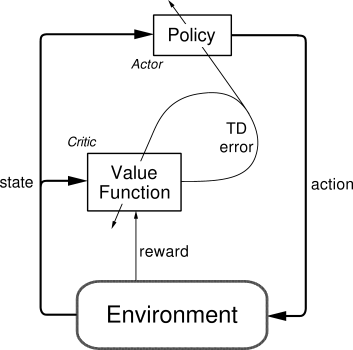
\includegraphics[width=75mm]{Figures/AC.png}
    \caption{Actor Critic Architecture}
    \label{fig:acarch}
\end{figure}

The \say{Advantage} of the advantage actor critic variants, refers to the use of the  advantage value as the output of the value function. The advantage value can be described as the relative value of any given action compared to the average value of all actions available in the current policy. It is formally defined as per the equation below where \(A^\pi(s,a)\) is the advantage function of an action at a given state, \(Q^\pi(s,a)\) is the optimal action-value function of an action at a given state and \(V^\pi(s)\) the optimal value function for any given state,
\[A^\pi(s,a) = Q^\pi(s,a) - V^\pi(s) \]

A2C (Advantage Actor Critic) \citet{YuhuaiWu17a2c} is a variant of the earlier A3C (Asynchronous Advantage Actor Critic) \citet{mnih2016asynchronous}. Both A2C and A3C use multiple workers to update the policy with the A3C variant using asynchronous workers in an attempt to improve computational efficiency. Further research \citep{YuhuaiWu17a2c} has shown that the synchronous workers of A2C agent actually perform better \say{Our synchronous A2C implementation performs better than our asynchronous implementations — we have not seen any evidence that the noise introduced by asynchrony provides any performance benefit. This A2C implementation is more cost-effective than A3C when using single-GPU machines, and is faster than a CPU-only A3C implementation when using larger policies.} \citep{YuhuaiWu17a2c}

\subsection{Long Short Term Memory} \label{section:lstm}
Recurrent Neural Networks \citep{RumelhartDavidE1986Lrbb} are an approach to processing sequential data such as event streams, video, time-series and other data that have long sequences, generally of few or one dimensions.  RNN's are prone to the vanishing or exploding gradient problem. In scenarios where the training data has long sequences then the gradients may tend towards zero, (vanish), or infinity (explode).  LSTM's \citep{Hochreiter1997}  resolve the vanishing gradient effect by connecting the hidden cells of the RNN to form  self-loops that can preserve the states across long sequences. The addition of the \say{forget gate} \citet{GersFelixA2000LtFC} introduced the ability to allow the time sequence to be controlled dynamically rather than as a fixed parameter.
\begin{figure}[h]
    \centering
    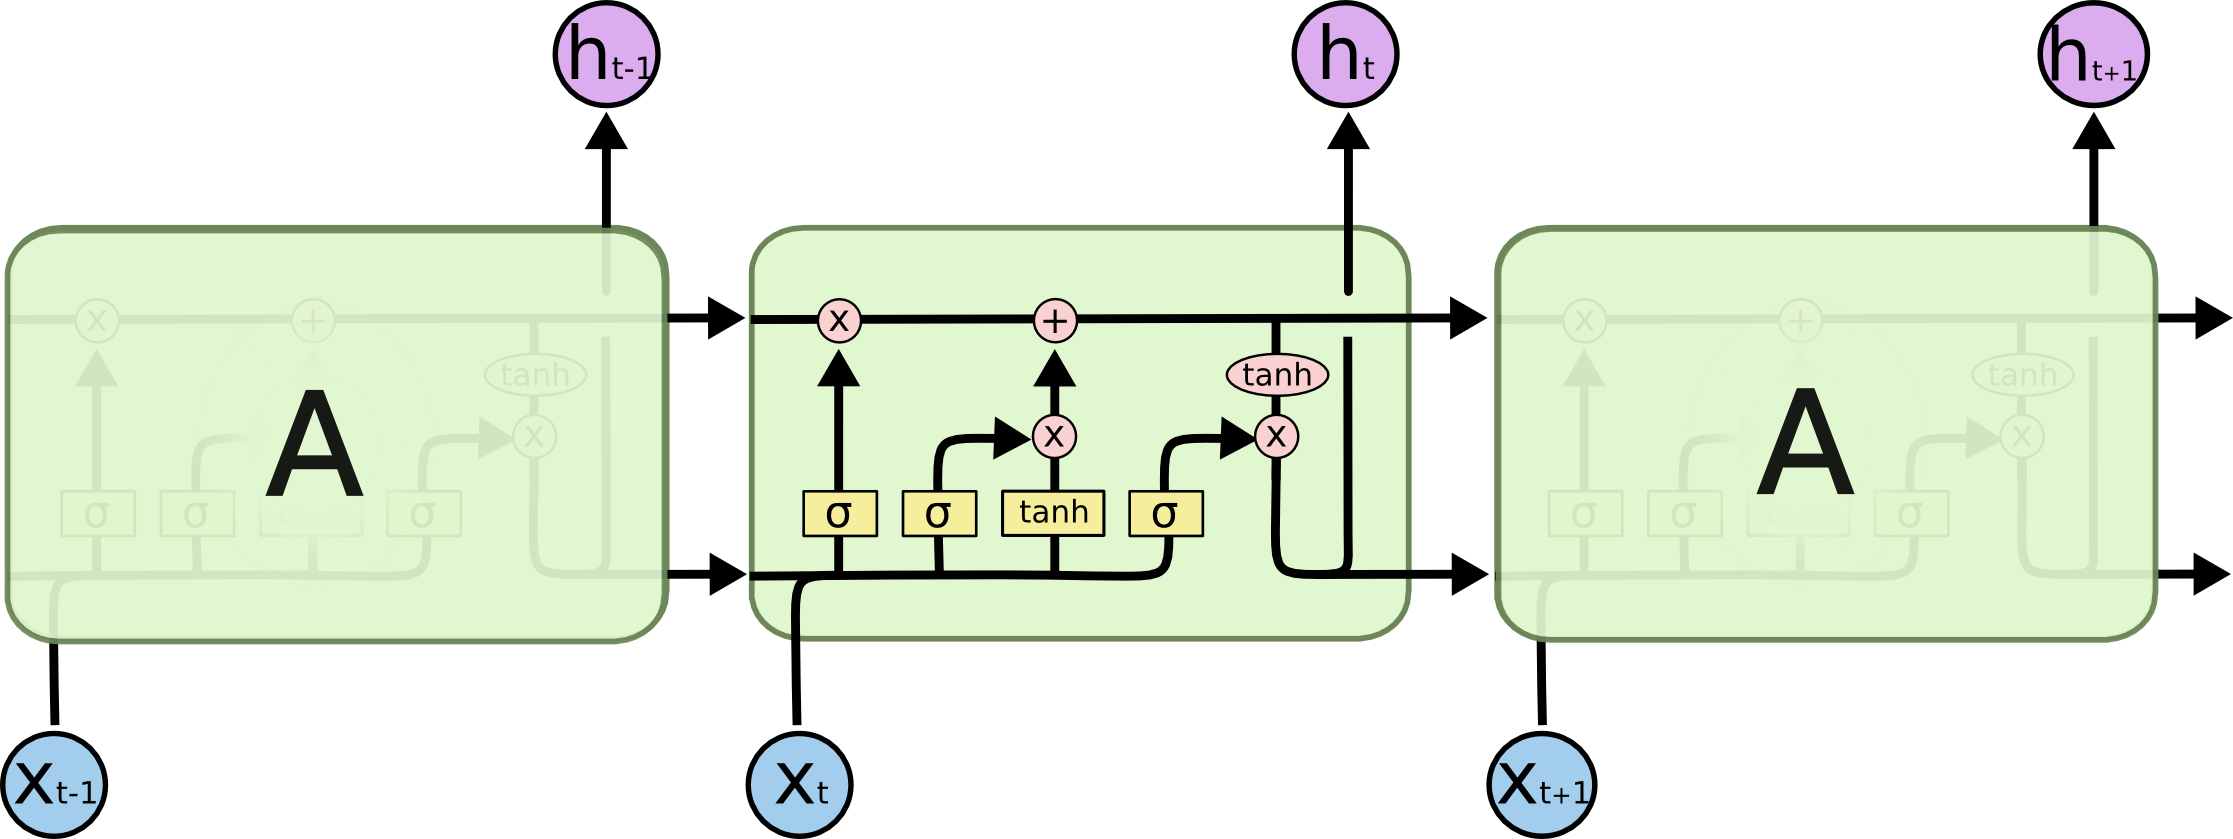
\includegraphics[width=100mm]{Figures/LSTM.png}
    \caption{LSTM State flow and gates}
    \label{fig:lstm}
\end{figure}

Figure \ref{fig:lstm} \citep{45500} shows the core concepts of an LSTM. Each LSTM cell has a an information flow or state represented by the lines passing through the cells.  Each cell has three neural nets that can either add or detract information from the state and a final fourth neural net decides what information is passed to the next cell. In the the portfolio allocation space, a possible example is where a sudden spike in asset price volatility may result in the gates discarding previous moving average prices as the volatility spike renders them meaningless.

\subsection{RL Frameworks}
There are several RL frameworks to choose from that assist in the creation of both agents and environments.  Open AI Gym \citep{1606.01540} was used in the implementation of this study. Open AI Gym is a widely used collection of environments and has a well documented API to create and publish custom environments. It is also compatible with most agent frameworks

StableBaselines \citep{stable-baselines} is a framework with implementations of most major SOTA agents and policies, including A2C and LSTM's. It is well documented with a API that allows for fine tuning of the agents and policies parameters. It also has a mature training and hyperparameter tuning component, RL Zoo \citep{rl-zoo}. Based on Tensorflow 1.15, StableBaselines is no longer actively maintained. It has been replaced by StableBaselines3 \citep{stable-baselines3}, based on Pytorch.  StableBaselines3, does have an A2C agent available, but it does not support RNN or LSTM policies as of yet. Other frameworks where considered, but for this study StableBaselines provided the functionality required.

\chapter{Related Work}
\label{chap:rel_work}
\section{Research Methods}
The literature for this paper was found via the following methods
\begin{itemize}
\item Online searches performed via the NUIG Library, Scopus and Scholar.
    \begin{itemize}
    \item Keywords include used singularly or in combination: Reinforcement Learning, Portfolio Management, Fintech, Investment, Trading Systems, Econometrics, Quantitative Finance.
    \item Filtering was performed using citation count, the relevance of the title and article abstracts, the date of publication, the citation counts of the authors, the count of article by the authors along with key metrics provided by each tool.
    \end{itemize}
\item Reviewing Journals found in JSTOR and Scimago.
\end{itemize}
\section{DRL  – Uses in Portfolio Management}
The following papers are addressed chronologically. The list is not a comprehensive set of all research in the field but is a representative set of DRL approaches relevant to portfolio management. A survey of portfolio selection techniques, not limited to reinforcement learning, was published in \citet{LiBin2014OpsA} and this along with the book by the same authors \citet{LiBin2016OPSP} have been used as a reference for this review

\citet{MoodyJohn1998Pfar} used recurrent reinforcement learning (RRL) algorithms. They also use the term \say{performance function} as a portfolio selection specific usage of the more general reinforcement learning \say{value function}. The performance functions used are \say{profit or wealth, economic utility, the Sharpe ratio and our proposed differential Sharpe ratio} \citep[p1]{MoodyJohn1998Pfar}. The Sharpe Ratio was a term that arose from William Sharpe’s paper \citep{SharpeWilliamF1964CAPA} but Sharpe went on to specifically describe it in the paper \citep{Sharpe94}. 

\citet{MoodyJohn1998Pfar} used the S\&P 500/TBill index as the benchmark for their simulation results for a 25-year period from 1970 to 1994.  In the conclusion they summarize the use of recurrent reinforcement learning as follows \say{Reinforcement learning algorithms find approximate solutions to stochastic dynamic programming problems and are able to do so on-line. Although it is possible to train the systems off-line using batch learning, we favour on-line reinforcement learning, as it is more efficient computationally. The learning algorithms we use are thus stochastic optimization methods. We utilize a simple but unique recurrent reinforcement learning (RRL) algorithm based on real-time recurrent learning (RTRL) that maximizes immediate rewards in an on-line mode} \citep[466]{MoodyJohn1998Pfar}. They also claim that the RRL approach \say{provides more stable results and higher profits and Sharpe ratios than does the Q-Learning algorithm for the 25-year out-of-sample period for the S\&P 500/TBill asset-allocation system.} \citep[467]{MoodyJohn1998Pfar}
 
Moody further builds on this in conjunction with Matthew Saffell \citet{MoodyJ2001Lttv}.  RRL is again used and \say{The need to build forecasting models is eliminated, and better trading performance is obtained. The direct reinforcement approach differs from dynamic programming and reinforcement algorithms such as TD-learning and Q-learning, which attempt to estimate a value function for the control problem. We find that the RRL direct reinforcement framework enables a simpler problem representation, avoids Bellman’s curse of dimensionality and offers compelling advantages in efficiency.} \citep[p875]{MoodyJ2001Lttv}. In the conclusion they find that an RRL approach outperforms Q-Learning \say{In this paper, we have compared the DR approach using RRL to the Q-learning value function method. We find that an RRL-Trader achieves better performance than a Q-Trader for the S\&P 500/T-Bill asset allocation problem} 

\citet{JiangZhengyao2017ADRL} presents a \say{financial-model-free Reinforcement Learning framework to provide a deep machine learning solution to the portfolio management problem} \citep[p1]{JiangZhengyao2017ADRL} . They refer to work of  \citet{MoodyJohn1998Pfar} and \citet{MoodyJ2001Lttv} and others and state \say{These RL algorithms output discrete trading signals on an asset. Being limited to single-asset trading, they are not applicable to general portfolio management problems, where trading agents manage multiple assets.} \citep[p.2]{JiangZhengyao2017ADRL}.

They propose \say{an RL framework specially designed for the task of portfolio management. The core of the framework is the Ensemble of Identical Independent Evaluators (EIIE) topology. An IIE is a neural network whose job is to inspect the history of an asset and evaluate its potential growth for the immediate future. The framework was tested using the polonix.com cryptocurrency exchange against three types of IIE, Convolutional Neural Network (CNN), Recurrent Neural Network (RNN) and Long Short Term Memory (LSTM) }\citep[p.3]{JiangZhengyao2017ADRL}.

In the conclusion they state \say{The profitability of the framework surpasses all surveyed traditional portfolio-selection methods, as demonstrated in the paper by the outcomes of three back-test experiments over different periods in a cryptocurrency market. In these experiments, the framework was realized using three different underlining networks, a CNN, a basic RNN and a LSTM. All three versions better performed in final accumulated portfolio value than other trading algorithms in comparison.} \citep[p.20]{JiangZhengyao2017ADRL}. In comparing the three IIE’s they state \say{LSTM had much lower scores than the CNN and the basic RNN. The significant gap in performance between the two RNN species under the same framework might be an indicator of the well-known secret in financial markets, that history repeats itself. Not being designed to forget its input history, a vanilla RNN is more able than a LSTM to exploit repetitive patterns in price movement for higher yields.} 

They also point out that there is room for improvement especially with regard to the volume of real-world trading examples \say{The main weakness of the current work is the assumptions of zero market impact and zero slippage. In order to consider market impact and slippage, large amount of well-documented real-world trading examples will be needed as training data}

\citet{ALMAHDI2017267} again build on the work of \citet{MoodyJohn1998Pfar} and \citet{MoodyJ2001Lttv}. They apply the \say{recurrent reinforcement learning (RRL) method with a statistically coherent downside risk-adjusted performance objective function to simultaneously generate both buy/sell signals and optimal asset allocation weights.} \citep[p267]{ALMAHDI2017267}. They point out that although \citet{MoodyJohn1998Pfar} and others discuss potential drawdown effects no study of the effects have been performed. To counter this they proposed to use \say{expected maximum drawdown E(MDD)} \citep[p267]{ALMAHDI2017267} as the performance function in place of the differentiated Sharpe Ratio used by \citet{MoodyJohn1998Pfar}.  They also constructed five asset portfolio using five of the most commonly traded exchange-traded funds from different asset categories. These assets (identified by their ticker symbols and fund names) are as follows: \citep[p271]{ALMAHDI2017267}.
\begin{itemize}
\item IWD: iShares Russell 10 0 0 Value 
\item IWC: iShares Micro-Cap 
\item SPY: SPDR S\&P 500 ETF 
\item DEM: WisdomTree Emerging Markets High Dividend 
\item CLY: iShares 10+ Year Credit Bond
\end{itemize}

In the conclusion they find \say{a) variable weight long/short portfolios outperform the equally weighted long/short portfolios; b) the RRL Calmar ratio based portfolios outperform the RRL Sharpe ratio based portfolios consistently; c) the E(MDD) RRL based trading system with market condition stop-loss retraining responds to transaction cost effects better and outperforms hedge fund benchmarks consistently.} \citep[p279]{ALMAHDI2017267}. They also state that \say{using RRL with the expected maximum drawdown based Calmar ratio results in a significantly superior performance and are more transaction cost resilient than the portfolios constructed with the Sharpe ratio.} \citep[p279]{ALMAHDI2017267}
 
The work of \citet{MoodyJohn1998Pfar} is again used as a baseline for \citet{ABOUSSALAH2020112891} and they propose that \say{To address the challenge of continuous action and multi-dimensional state spaces, we propose the so called Stacked Deep Dynamic Recurrent Reinforcement Learning (SDDRRL) architecture to construct a real-time optimal portfolio.} \citep[p1]{ABOUSSALAH2020112891}. The Sharpe Ratio is used as the performance value and in addition, the authors used a hyperparameter tuning method given the sensitivity of machine learning algorithms to the hyperparameter settings \say{Therefore, we equipped SDDRRL with the ability to find the best possible architecture topology using an automated Gaussian Process ( GP ) with Expected Improvement ( EI ) as an acquisition function. This allows us to select the best architectures that maximize the total return while respecting the cardinality constraints.} \citep[p1]{ABOUSSALAH2020112891}. The model was tested against a set of stock from the S\&P500 from January 1st 2013 to July 31st 2017.

The authors do not compare the performance of the notional investment to previous works but do state that \say{The optimized number of time-stacks was found to be approximately equal to 5 or 6, leading to annualized returns around 20\% throughout our testing period. However, the size of the training and testing windows should be optimized and was left for future work.}\citep[p10]{ABOUSSALAH2020112891}.

They also state that \say{different policy neural network architectures have different investment strategies over the same period of time, which could be interpreted as having five different portfolio management experts. By aggregating the decisions coming from these experts, we can be more robust in the face of market fluctuations.} \citep[p12]{ABOUSSALAH2020112891}. They suggested future work for \say{aggregating the decisions through the use of either ensemble methods e.g. Bagging, Boosting or possibly the Multi-Armed Bandit approach}.

\citep{BaileyDavidH2012Tsre} propose a variation of the Sharpe Ratio, the \say{Probablistic Sharpe Ratio} \citep[p.3]{BaileyDavidH2012Tsre} or PSR. They argue that the \say{Sharpe ratio is a deficient measure of investment skill} and that \say{non-Normality may increase the variance of the Sharpe ratio estimator, therefore reducing our confidence in its point estimate} \citet[p.4]{BaileyDavidH2012Tsre}. The PSR attempts to address the deficiencies of the Sharpe Ratio under non-Normal conditions by a identifying a the length of the track record that best reflect the portfolio performance. The conclude \say{despite Sharpe ratio’s well-documented deficiencies, it can still provide evidence of investment skill, as long as the user learns to require the proper track record length.} \citep[p.15]{BaileyDavidH2012Tsre}

\section{Goal Based Inverse Reinforcement Learning}
A different approach is discussed in Chapter 11 of \citet{DixonMatthewF2020MLiF} and also in \citet{dixon2020glearner}. The approach is goal based and referred to by the authors as a G-Learner. The G-Learner is combined with inverse reinforcement learning. Inverse reinforcement learning does not observe the reward but instead seeks to learn a reward function based on the behaviour of the agent and derive the optimal policy. The resulting algorithm is referred to by the authors as \say{GIRL (G-learning IRL)} \citep[p5-18]{dixon2020glearner}. This approach involves no deep learning, so although very interesting, was not used in this study as Deep Reinforcement Learning is a personal learning objective of this thesis.                                                                                         

\section{FinRL - DRL for Finance}
FinRL is described in \citet{finrl2020}. The library aims to provide a \say{library that streamlines the development of stock trading strategies. FinRL provides common building blocks that allow strategy builders to configure stock market datasets as virtual environments, to train deep neural networks as trading agents, to analyze trading performance via extensive backtesting, and to incorporate important market frictions.} \citet[p.2]{finrl2020}

This library was not directly used in this study, as it is based on the library StableBaseline3 \citep{stable-baselines3} which does not support LTSM or RNN policies for any of the supported agents. However, the framework and associated papers where used as a reference point for the implementation.         

\chapter{Data}
\label{chap:data}
The following section discusses the data required for the study, the sources of the data and how the data was prepared.
\section{Source Data and Preparation}
Three sets of data where required for this study for the period 2008 to 2020.
\subsection{S\&P 500 Constituents}
The constituent stocks  of the S\&P 500 index where provided by S\&P 500 Indices, under academic license. The data included constituents of other S\&P indices and was filtered using the index key.

The constituents of the S\&P 500 are selected based on market capitalization and at any given time may have more than 500 stocks if the selected companies have one or more publicly traded share classes included the market capitalization.  The constituents are updated regularly and over the period of the study in excess of 720 companies where included in the index.  As the input layer of the A2C agent requires a fixed dimension, then the price data for those  that where not in the S\&P 500 on any given day where inserted and all values set to 0. As per the \ref{section:stepfunc}, where allocation are made to these stocks then the allocation is moved to cash and added back to the portfolio value.


\subsection{S\&P 500 Daily Returns}
The daily returns of the S\&P 500 was included in the constituent data provided,  but only on a quarterly basis. The additional daily returns data required was sourced from Yahoo Finance \citep{YahooFinance} using the yfinance python API \citep{Ranaroussi2019} via the key \say{\^GSPC}. 
\subsection{S\&P 500 Constituents Daily Pricing}
The daily price data of the constituent stocks where initially sourced from Yahoo Finance \citep{YahooFinance} using the yfinance python API \citep{Ranaroussi2019}. However, several data quality issues such as missing time periods and corrupted values rendered this source unsuitable. In addition Yahoo Finance only provide historical data for companies that still are still trading. Over the period of study, new companies formed, existing ones ceased, merged with others or where brought back into private ownership. An alternative source was used instead, \citet{SimFin2020} which overcame these issues.

Some stock price data was still missing for short periods of time and for the purposes of this study the missing data was replaced with the last known days prices but with trade volumes set to 0.  There are issues with this approach if trying to use this data to trade profitably but for the purposes of this study, this approach was adequate.

Intra-day prices are not needed in this study as  it is focused on longer term investments maximising the return of a portfolio of assets rather than a short term  individual stock investment.
\section{Technical Indicators} \label{section:technical indicators}
The raw price data of a stock, including high, low, close, adjusted close and daily volumes, on any given day are poor indicators of whether the stock should be sold or bought, in what quantity or just held. 

Technical indicators are used to overcome the shortcoming of simple price and volume data. All technical indicators where calculated using the ta python library  \citep{ta-lib}.
The simplest of these is the daily return. This is  the difference in closing price over the preceding day and is used in this study.
Technical indicators are generally used in combination to make trade decisions hence a selection of  common indicators are also used. These are listed in terms momentum, volatility and trend.
\begin{itemize}
    \item Momentum - indicators of the speed at which a stock price is changing either up or down. The Stochastic Oscillator was used to signal momentum.
    \item Volatility - indicators used to establish how volatile a stock is. Bollinger Bands including moving average, high band, low band and high and low band indicators where used to as the volatility indicator.
    \item Trend - indicators of the upward or downward trends over various periods. Exponential Moving average (50 and 200 day) and Moving Average Convergence-Divergence where used as the trend indicators.
    \item Volume - On Balance Volume was used as the volume indicator.
\end{itemize}

\chapter{Implementation} \label{chap:methodology}
\section{Reward Function Selection} \label{section:rewardfunc}
Possible rewards functions include absolute Portfolio Value, Portfolio Value change per step or Cumulative Returns. The issue with all these and similar rewards is that they do not take into account prevailing market conditions and are often referred to as Beta returns. Beta returns can be defined as returns generated via general market conditions. Alpha returns are those attributed directly to a decision made by the investor.  For example, in a general rising market a well balanced Portfolio can expect positive Beta returns in line with the overall market conditions. Alpha returns may be achieved, for example, by analysis of the market and identifying  a stock that is predicted to rise or fall in price  faster than the overall market, and then trade to take advantage of this prediction.

The reward function should attribute Alpha returns to the agent and discount Beta returns. Hence, the excess return over the S\&P 500 has been used, where the S\&P 500 returns are considered the Beta. In a rising market a reward will be attributed to the learner where the returns are greater than the S\&P 500 returns. In a falling market a reward can be attributed to the learner even if the returns are negative, as long as the loss is less than a negative return of the S\&P 500 i.e. we can attribute a positive reward when the learner is minimising losses. 

Using risk ratios such as Sharpe, Probalistic Sharpe, Calmar etc was considered for this study, but was not implemented and instead focused on excess over benchmark.

\section{Environment}
As stated, the environment was constructed using the  OpenAI Gym framework \citet{1606.01540}.  The step function is described below. Note the below only includes the core step functions. Other functions, including maintaining action, weight and portfolio history are not specified here for the sake of brevity. Full source code can be found at \citet{KeithBinesThesis2021} in \newline SB2/PortfolioAllocation/PortfolioAllocationGym/envs/Portfolio.py 
\subsection{Step Function} \label{section:stepfunc}
\begin{itemize}
\item Until Terminal is True
    \begin{itemize}
    \item Get Current Day
    \item If Current Day is greater than Last Day 
        \begin{itemize}
        \item set terminal to true
        \item Return reward (excess returns), state (last day price data) and terminal (True)
    \end{itemize}
    \item Else if Current day is First Day and Random Sample is True
    \begin{itemize}
        \item resample data
    \end{itemize}
    \item End If
    \item Distribute the Actions as \textit{Weight - Action / Sum of Actions}
    \item Allocate weights to each stock - \textit{Weight * Portfolio Value / Closing Prices}
    \item Move funds with 0 price to cash
    \item For allocations of 0, move the previous days value to cash (stock is liquidated)
    \item Sum all cash and add it Portfolio Value
    \item Get returns proportional to  the weights
    \item Get excess returns against benchmark
    \item Return reward (excess returns), state (next day price data) and terminal (False)
    \end{itemize}
\end{itemize}

\section{Agent and Policy}
The StableBaseline \citep{stable-baselines} A2C implementation with a layer normalized LSTM policy and MLP feature extractor was used for the agent architecture. The agent definition can be found the jupyter notebook in  SB2/SB2\_AC2\_MLP.ipynb

\chapter{Experimental Settings} \label{chap:experimental}
During initial environment construction and testing various reward functions where experimented with. As per \ref{section:rewardfunc}, attributing the reward to the agents actions is only really possible using the excess over the benchmark. 

Once some repeatable stability in the agent training was achieved hyperparameter tuning and training was then carried out as detailed below. This was an iterative process and the agent and environment where modified several times during the course of the experiments.

\section{Hyperparameter Tuning}
Hyperparmeter tuning was carried out using the RL-Zoo \citep{rl-zoo}. RL Zoo is a template that can be modified to meet the needs of custom environments.  The modification required for this study cane be found in the forked github repository  at \citet{KeithBinesRLZoo2021}  The following table describes the final set of parameters that where tuned along with the tuned parameters. The final tuning process was completed over 100 trials. Although there are tens of thousands combinations of the categorized parameters, 100 trials was choosen for the final session based on the number of trails pruned and variance of target objectives in previous sessions. The parameters sets used in the trials are as per table \ref{table:hyperparamvals}

\begin{table} [h]
\begin{tabular}{|l|l|}
\hline
\textbf{Parameter} & \textbf{Values Tested }\\
\hline
Gamma & 0.9, 0.9999\\
Steps & 1, 5, 10, 30, 90\\
\hline
Learning Rate Schedule & linear. constant \\
\hline
Learning Rate & 0.0001, 0.0007, 0.001, 0.01\\
\hline
Entropy Co-Efficient & 0.00000001, 0.000001, 0.0001, 0.1\\
\hline
Value Function Co-Efficient & 0, 0.25, 0.5, 0.75, 1\\
\hline
Max. Gradient Normalization & 0.3, 0.7, 1, 2, 5\\
\hline
LSTM Cells & 64, 128, 256\\
\hline
Activation Function & TanH, Relu, Leaky Relu\\
\hline
\end{tabular}
\caption{HyperParameter Values} \label{table:hyperparamvals}
\end{table}

The StableBasleine \citep{stable-baselines} LSTM policy allows for the specification LSTM, Policy and Value Function neural nets.  Some basic architectures where included in the hyper parameters sets as per table \ref{table:hyperparamna}

\begin{table}[h]
\begin{tabular}{|l|l|l|}
\hline
\textbf{LSTM Layer} & \textbf{Policy Layers} & \textbf{Value Function Layers} \\
\hline
8 & [32, 32] & [32, 32] \\
\hline
64 & [32, 32] & [32, 32] \\
\hline
128 & [64, 64] & [64, 64] \\
\hline
64 & [64, 64, 64] & [64, 64]\\
\hline
128 & [128, 128, 128] & [128, 128, 128] \\
\hline
\end{tabular}
\caption{HyperParam Network Architectures} \label{table:hyperparamna}
\end{table}

\subsection{Tuned Parameters} \label{section:tunedHP}
The tuned parameters used where
\begin{itemize}
    \item gamma: 0.9999
    \item steps: 1
    \item learning rate schedule : linear
    \item learning rate: 0.001
    \item Entropy Co-Efficient: 0.1
    \item Value Function Co-Efficient : 0
    \item Max Gradient Normalization : 5
    \item LSTM Cells : 128
    \item Activation Function : TanH,
    \item Network: LSTM - 128, Policy [256, 256], Value Function [256, 256]
\end{itemize}

\section{Model Training}
The model was trained using the parameters from \ref{section:tunedHP}

Training was run several times with the timestep set as a multiplier of stepping through the entire period i.e. \textit{n * environment trading days}.  During training it was found that values of \textit{n} in excess of 100 caused the reward function to return NaN's.  LSTM's resolve the issue of the vanishing gradient but are still prone to exploding gradients during training, resulting in rewards of infinity returned by the framework as a NaN. This could also be an unresolved defect in the step function.

Training was performed with a sample size of 100 stocks, over the period 2008 to 2017 with an initial investment of 1m. Stocks where selected at random as per \ref{section:stepfunc}.
Monitoring via Tensorflow tensorboard, did not really show any real pattern in the training, however training with \textit{n} as 40 seemed to be the most stable. The episode rewards, advantage and discounted rewards are shown in \ref{fig:tensorboard}. 
Using random samples during training is based on the hypothesis that the agent will not learn which stocks increased the excess returns but instead learn from the technical indicators. However this does mean the possible returns are going to vary with each step as new stocks are sampled, and this may explain why the graphs in \ref{fig:tensorboard} show no particular learning pattern.

However, for the 40 steps through the training data, the agent did not exceed the index returns on only two occasions. 

\begin{figure}[h]
    \centering
    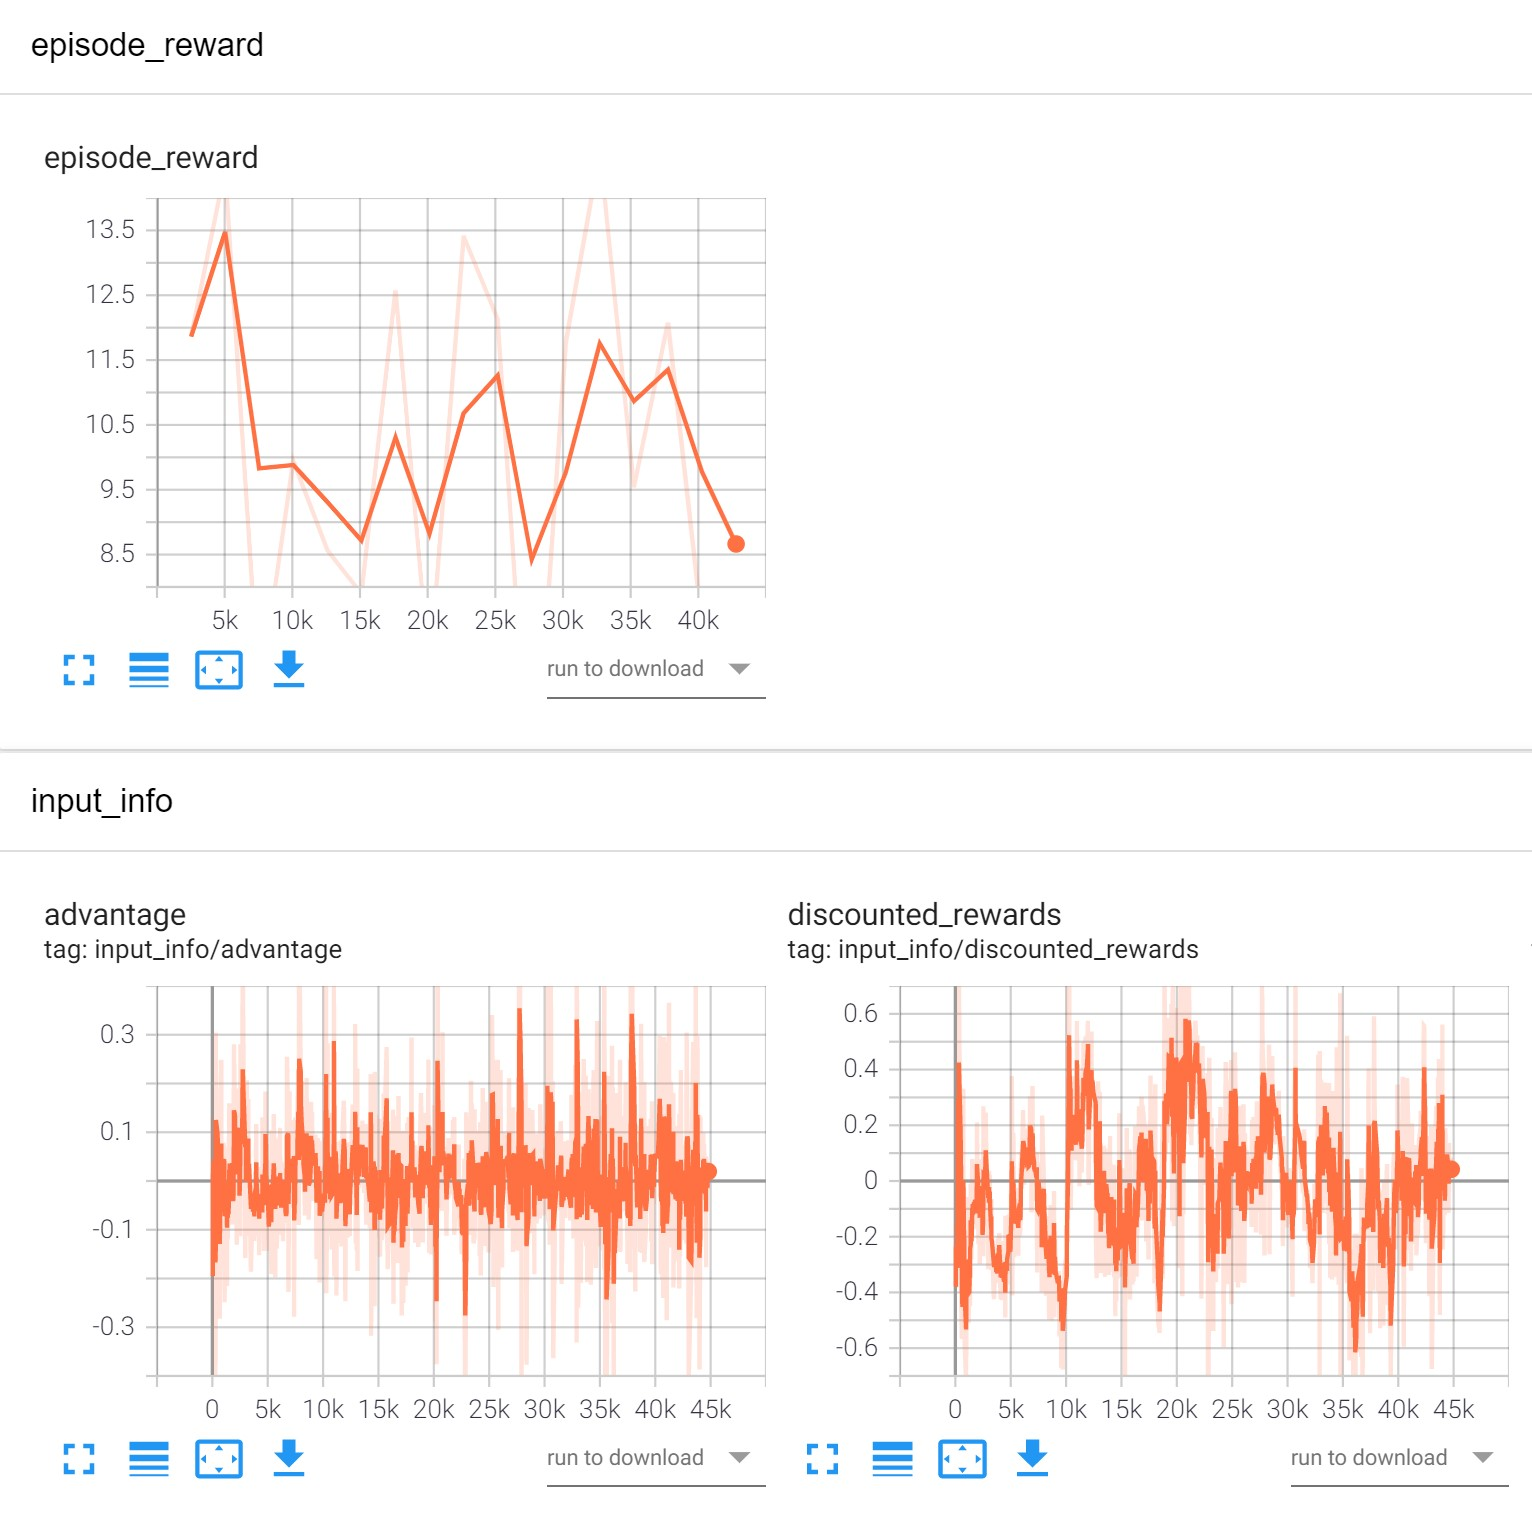
\includegraphics[width=15cm]{Figures/Training.jpg}
    \caption{Training Graphs}
    \label{fig:tensorboard}
\end{figure}



\chapter{Results}
\label{chap:resutls}
A second evaluation environment was created, for the period 2018 to 2020, with 100 stocks selected by highest stock price at the beginning of the period and with an initial investment of 1m.

An untrained agent was first tested against the evaluation environment followed by the trained agent.
The mean reward and stand deviation of rewards was calculated and the results are shown in \ref{table:untrained} and \ref{table:trained}

\begin{table}[h]
    \centering
    \begin{tabular}{|l|l|l|l|l|l|}
    \hline
     Step & Sharpe & Index & Mean Excess & Cumulative& Portfolio\\
     \-\ & Ratio & Returns & Returns & Returns & Value\\
    \hline
    1 &2.113 & 64.277 & 0.994  & 30.603 & 1,306,031.22\\
    \hline
    2 &2.233 & 64.277 & 1.277  & 32.975 & 1,329,752.52\\
    \hline
    3 &2.105 & 64.277 & 0.975  & 30.393 & 1,303,926.48\\
    \hline
    4 &2.121 & 64.277 & 1.014  & 30.748 & 1,307,481.55\\
    \hline
    5 &2.303 & 64.277 & 1.442  & 34.484 & 1,344,841.85\\
    \hline
    6 &2.363 & 64.277 & 1.584  & 35.797 & 1,357,969.92\\
    \hline
    7 &2.406 & 64.277 & 1.685  & 36.690 & 1,366,904.62\\
    \hline
    8 &2.400 & 64.277 & 1.671  & 36.553 & 1,365,527.06\\
    \hline
    9 &2.392 & 64.277 & 1.651  & 36.372 & 1,363,722.47\\
    \hline
    10 &2.394 & 64.277 & 1.656  & 36.419 & 1,364,192.87\\
    \hline
    \end{tabular}
    \caption{Untrained A2C Agent}
    \label{table:untrained}
\end{table}

Untrained Agent: Mean Reward:5.83 +/- 1.77

\begin{table}[h]
    \centering
    \begin{tabular}{|l|l|l|l|l|l|}
    \hline
     Step & Sharpe & Index & Mean Excess & Cumulative& Portfolio\\
     \-\ & Ratio & Returns & Returns & Returns & Value\\
    \hline
    1 & 2.394 & 64.277 & 1.657 & 36.428 & 1,364,283.82\\
    \hline
    2 & 2.395 & 64.277 & 1.659 & 36.447 & 1,364,469.36\\
    \hline
    3 & 2.392 & 64.277 & 1.651 & 36.372 & 1,363,718.29\\
    \hline
    4 & 2.385 & 64.277 & 1.634 & 36.227 & 1,362,271.62\\
    \hline
    5 & 2.364 & 64.277 & 1.586 & 35.800 & 1,358,004.98\\
    \hline
    6 & 2.358 & 64.277 & 1.571 & 35.670 & 1,356,704.41\\
    \hline
    7 & 2.359 & 64.277 & 1.574 & 35.696 & 1,356,962.39\\
    \hline
    8 & 2.364 & 64.277 & 1.585 & 35.795 & 1,357,951.55\\
    \hline
    9 & 2.371 & 64.277 & 1.603 & 35.947 & 1,359,469.56\\
    \hline
    10 & 2.378 & 64.277 & 1.619 & 36.094 & 1,360,944.13\\
    \hline
    \end{tabular}
    \caption{Trained A2C Agent}
    \label{table:trained}
\end{table}
Trained Agent: Mean Reward:6.05 +/- 0.12

The trained agent does perform slightly better than the untrained agent and there is less deviation in the returns. This does suggest that there is some active policy being learned, but is not enough evidence to say this is proof of a learned policy.
This could be due to the sample selection criteria. The 100 highest prices stocks may be more likely to perform strongly and hence even a random agent can make a decent return. The Sharpe ratio of both the untrained agents is between 2.1 and 2.4 and the trained agents is fairly constant at 2.3. Sharpe ratio's approaching 3 tend to indicate a portfolio with a good risk:reward ratio and this may provide evidence that it is the initial stock selection that is driving the bulk of the excess returns.  The slight difference in the trained and untrained agents could be the result of an active learned policy allocating funds selectively.

\chapter{Conclusion}
\label{chap:conclusion}

There is not enough evidence in this study to definitively declare that the agent has learned a policy that can be attributed Alpha returns consistently in excess of the S\&P 500 index.  However, there is some indication that some advantage is being gained from the trained agent.

Further study could involve the following steps.
\begin{itemize}
    \item Using a larger sample size of stocks and training the agents against more specific indexes. The S\&P 500 is a broad spectrum of the largest companies by design, so as to reflect the US market in general.  As such it may be too general to easily train an agent against it. It may be more fruitful to select stocks of the same asset class, and including those not in the S\&P 500 and from countries outside of the US. Along with using an index specific to  that asset class may result in better training performance. Such indices, however, are generally only available on a paid license basis, and as such was not a strategy this study could take.
    \item Detailed Statistical Correlation.  A detailed statistical correlation of the input features i.e. the technical indicators, and how and if they correlate to both the stocks performance and the actions taken by the agent has not been  performed. This step was planned but was not performed in time for the submission date.
    \item HyperParameter Tuning. A more detailed tuning stage and study of the agents network architecture may increase the performance of the agent. During training the rewards where calculated as NaN. This is an indication that the  the network architecture requires further refinement. It should be stated that the NaN could also be a defect in the environment step function itself.
    \item Comparison to other Agents and Policies.  No other agent architectures, such as DQN, PPO TRPO, TD3 and others have been performed. In addition no comparison to other policies such as RNN or GRU have been performed either.  Such comparisons may help provide evidence to help prove or disprove the hypothesis.
    \item Reward Function. Reinforcement Learning is very dependent on the reward function.  The reward function is the daily excess returns of the portfolio over the S\&P 500 index. This may be too simple a reward to use for effective training. Using a logarithmic mean return, or a mean return over a fixed time or even a dynamic time period to reflect market cycles could provide a better reward function.
    \item Multi Objective. Training the agent with multi-objectives such as the Sharpe Ratio and the excess returns may also result in an increase in the agent performance.
\end{itemize}

As already state, the results of this study neither prove or disprove that the agent learned an effective policy. However, there are some indications that an effective policy is present. Related works identified in Chapter \ref{chap:rel_work} also show that DRL and other approaches such as GIRL are effective techniques. It is difficult to prove that any of these have been actually effective beyond academia and used to return profit in a commercial setting. If this is the case, then it may well be that organisations using such techniques keep it a closely guarded secret to gain a competitive advantage,



%%%%%%%%%%%%%%%%%%%%%%%%%%%%%%%%%%%%%%%%%%%%%%%%%%%%%%%%%%%%%%%%%%%%%%%%%%%%%%%%
\bibliographystyle{plainnat}                  % to give author-year style
\renewcommand{\bibname}{References}           % change default name Bibliography to References
\bibliography{references}                     % References file, references.bib
\addcontentsline{toc}{chapter}{References}    % add References to TOC


%\appendix
%\chapter{Appendix-A-Jupyter Notebook} 
%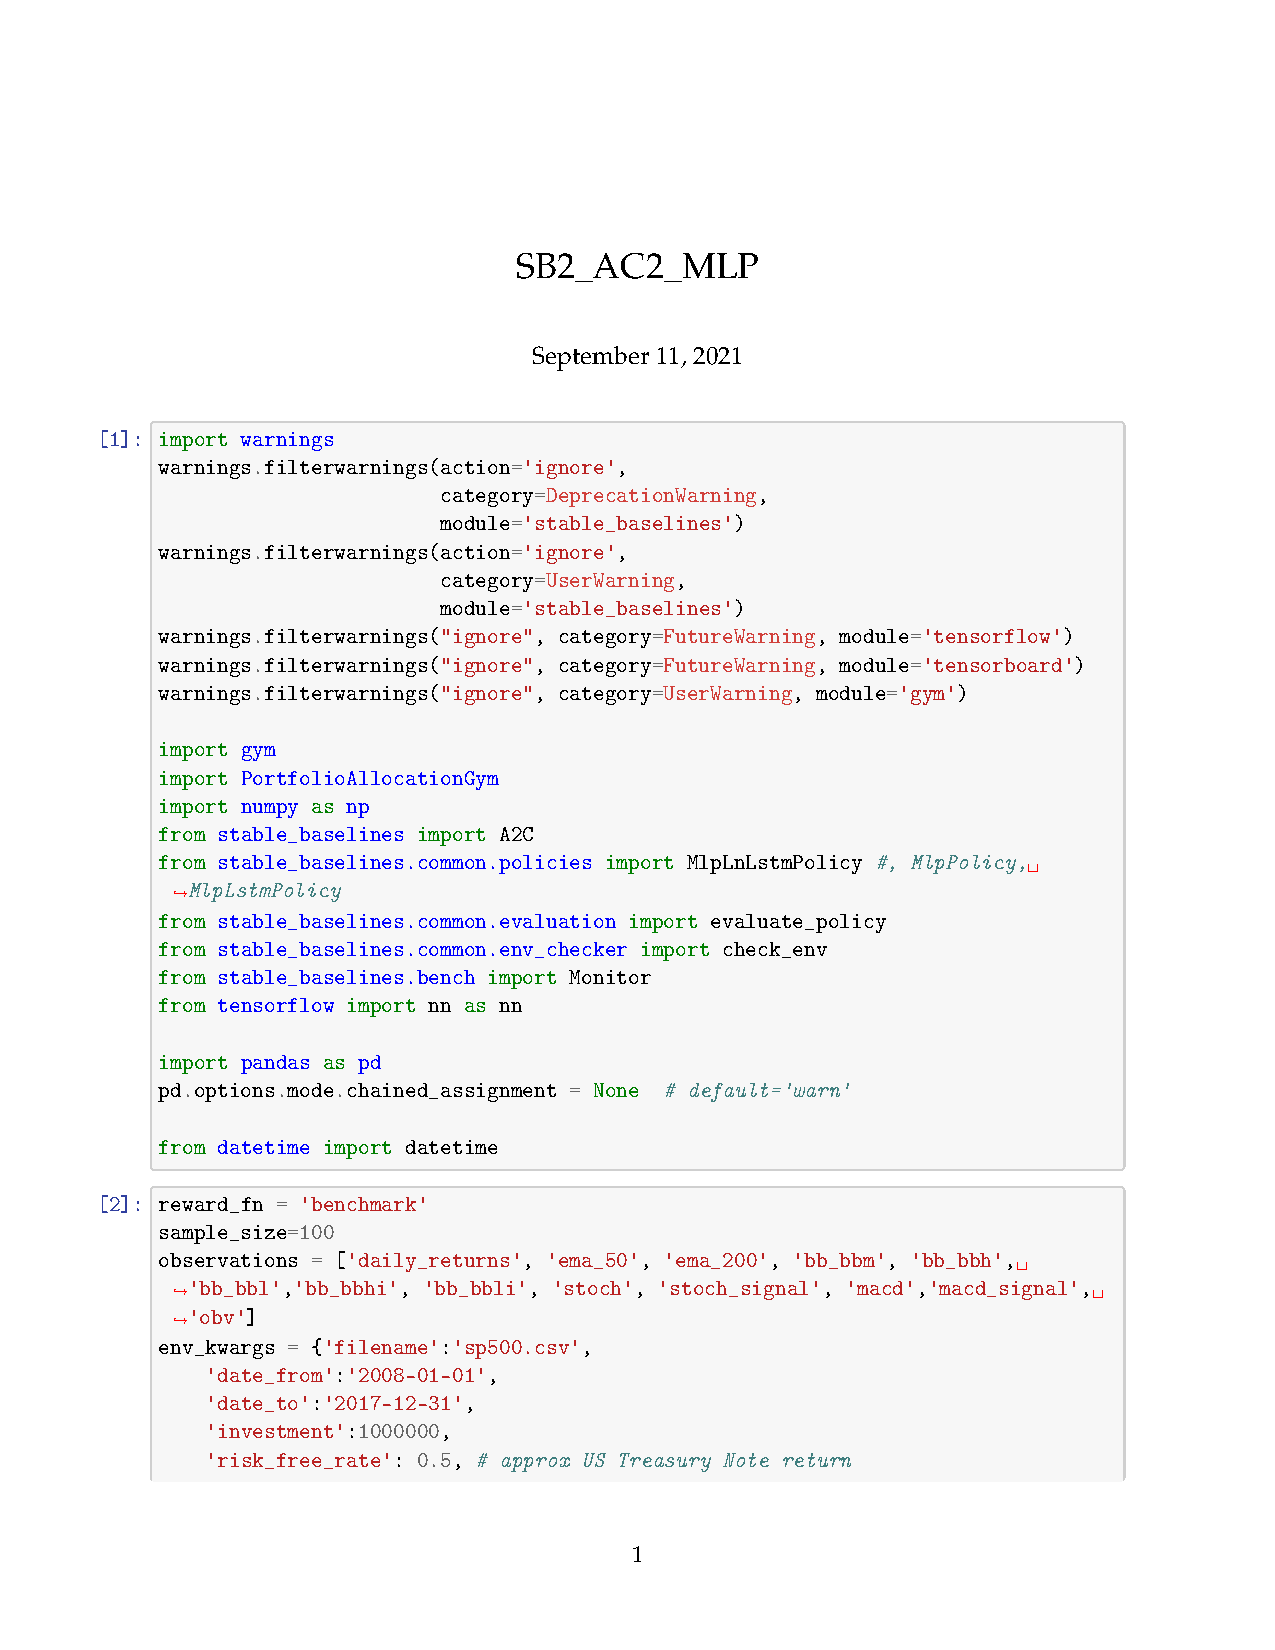
\includepdf[pages=-,pagecommand={},width=\textwidth]{Figures/Notebook.pdf}


\end{document}
